\documentclass[letterpaper,12pt]{article}
\usepackage[top = 1in, bottom = 1in, left = 0.5in, right = 1in]{geometry}
\usepackage{inputenc}
\usepackage{graphicx}
\usepackage{amsmath}
\usepackage{amsfonts}
\usepackage{caption}
\usepackage{color}
\usepackage{listings}
\usepackage[framed,numbered,autolinebreaks,useliterate]{mcode}
%opening
\author{Gowtham Garimella}

\makeatletter
\newcommand\ackname{Acknowledgements}
\if@titlepage
  \newenvironment{acknowledgements}{%
      \titlepage
      \null\vfil
      \@beginparpenalty\@lowpenalty
      \begin{center}%
        \bfseries \ackname
        \@endparpenalty\@M
      \end{center}}%
     {\par\vfil\null\endtitlepage}
\else
  \newenvironment{acknowledgements}{%
      \if@twocolumn
        \section*{\abstractname}%
      \else
        \small
        \begin{center}%
          {\bfseries \ackname\vspace{-.5em}\vspace{\z@}}%
        \end{center}%
        \quotation
      \fi}
      {\if@twocolumn\else\endquotation\fi}
\fi
\makeatother

\newcommand{\executeiffilenewer}[3]{%
\ifnum\pdfstrcmp{\pdffilemoddate{#1}}%
{\pdffilemoddate{#2}}>0%
{\immediate\write18{#3}}\fi%
}
\newcommand{\includesvg}[1]{%
\executeiffilenewer{#1.svg}{#1.pdf}%
{inkscape -z -D --file=#1.svg %
--export-pdf=#1.pdf --export-latex}%
\input{#1.pdf_tex}%
}

\title{EN.530.603 Applied Optimal Control \\HW \#3 Solutions}
\graphicspath{{./figures/}}
\begin{document}
\maketitle

\begin{enumerate}

  %%%%%%%%%%%%%%%Question 1%%%%%%%%%%%%%%%%%%%%%%%%
  \item Given system dynamics:
  \begin{align*}
   \dot x_1(t) &= x_2(t)\\
   \dot x_2(t) &= -a x_2(t) + u(t) \\
   a > 0 \quad |u(t)| &\le 1 \quad x(t_f) = 0\\
  \end{align*}
  To minimize:
  \begin{align*}
   J = \int_{t_0}^{t_f} \gamma + |u(t)| dt \quad \gamma > 0\\
  \end{align*}
  \begin{enumerate}
   \item The Hamiltonian and adjoint equations are as follows:
   \begin{align*}
    H &= \gamma + |u| + \lambda_1 ( x_2) + \lambda_2 (-a x_2 + u)\\
    \dot \lambda &= -\nabla H_x\\
    \Rightarrow \begin{bmatrix}
                 \dot \lambda_1\\
                 \dot \lambda_2\\
                \end{bmatrix} &= 
                \begin{bmatrix}
                 0 \\
                 -\lambda_1 + a \lambda_2\\
                \end{bmatrix}\\
    \nabla H_u &= \pm 1 + \lambda_2 \quad \text{(Does not provide u)}\\
    H^*_u &= |u| + \lambda_2 u \quad \text{(Choose u to minimize this)}\\
    \Rightarrow u &= \begin{cases}
                      -1 & \mbox{if}\enskip \lambda_2 > 1\\
                      0 & \mbox{if}\enskip 1 > \lambda_2 > -1\\
                      1 & \mbox{if}\enskip -1 > \lambda_2 \\
                     \end{cases}
   \end{align*}
   \item From the dynamics of the lagrange multipliers:
   \begin{align*}
    \lambda_1 &= c_1\\
    \lambda_2 &= c_2 e^{at} + \frac{c_1}{a}\\
   \end{align*}
   From the Boundary conditions, since the final time is free,
   \begin{align*}
    H(t_f) &= 0 \quad \Rightarrow \gamma + |u_f| + \lambda_{2f} u_f = 0\\
    \Rightarrow \lambda_2(t_f) &= \begin{cases}
                                  -(1+\gamma) &\mbox{if } u_f = 1 \\
                                  (1+\gamma) & \mbox{if } u_f = -1\\
                                 \end{cases}
   \end{align*}
   $u_f$ cannot be equal to zero in the above equation. Given that $\lambda_2(t)$ is exponential,
and the final value is either greater than 1 or less than -1, there can be atmost \textbf{two
switches}. So the optimal control sequences are: \{-1,0,1\} \{0,1\} \{1\} \{1,0,-1\} \{0,-1\} \{-1\}
 
   \item The singular points where the control becomes undefined is given when $\lambda_2 =
\{-1,1\}$. Given the form of $\lambda_2$ as:
   \begin{equation*}
    \lambda_2 = c_2 e^{at} + \frac{c_1}{a}\\
   \end{equation*}
  $\lambda_2$ is continuously increasing or decreasing unless $c_2 = 0$ in which case the boundary
conditions ensure that:
  \begin{equation*}
   \lambda_2 = \lambda_2(t_f) = \pm (1 + \gamma)
  \end{equation*}
  which is not any of the singular values. Thus the value of $\lambda_2$ cannot stay at the singular
values for any time interval. Thus there are no \textbf{singular intervals}.
  
  \item To determine the optimal control law we look at the curves with no switching:
   \begin{enumerate}
    \item u = -1 always. Then 
    \begin{align*}
     \dot x_2(t) &= -a x_2 - 1 \quad x_{2f} = 0\\
     x_2(t) &= (1/a) [e^{-a(t-t_f)} - 1]\\
     \dot x_1(t) &= x_2 \quad x_{1f} = 0\\
     x_1(t) &= (1/a) [(1/a)(1 - e^{-a(t-t_f)}) - (t-t_f))]\\
     \Rightarrow x_1(t) &= \frac{1}{a^2} [-ax_2 + log(ax_2 + 1)] \quad x_2 > (-1/a)\\
    \end{align*}
    \item u = 1 always. Then similar to above,
    \begin{align*}
      x_1(t) = \frac{-1}{a^2} [ax_2 + log(1 - ax_2)] \quad x_2 < (1/a)\\
    \end{align*}
    \item u = 0. Then
    \begin{align*}
     \dot x_2 &= -a x_2 \quad \dot x_1 = x_2 \\
     \Rightarrow x_1 &= -(x_2 - x_{20})/a  + x_{10}
    \end{align*}
    This is just a straight line with slope (-1/a).
   \end{enumerate}
  \end{enumerate}
   These combine to provide the switching curves shown in Fig[\ref{fig1}]. The general family of curves for u = \{1,-1, 0\} are
plotted in Fig[\ref{fig2}]. Based on the family of curves we come up with possible set of subsequences for the optimal control law presented below. Some example scenarios are presented in Figures[\ref{fig3}][\ref{fig4}]
    \begin{align*}
     u = \begin{cases}
          \{-1,0,1 \} \mbox{ or } \{0,1 \} & \mbox{if } x_{10} < \frac{1}{a^2} [-ax_{20} + log(1 + ax_{20})] \enskip\&\enskip x_20 \ge 0\\
          \{-1,0,1 \}  & \mbox{if } x_{10} < \frac{-1}{a^2} [ax_{20} + log(1 - ax_{20})]\enskip\&\enskip x_{20} \le 0\\
          \{1,0,-1 \} \mbox{ or } \{0,-1 \} & \mbox{if } x_{10} > \frac{-1}{a^2} [ax_{20} + log(1 - ax_{20})] \enskip\&\enskip x_{20} \le 0\\
          \{1,0,-1 \}  & \mbox{if } x_{10} > \frac{1}{a^2} [-ax_{20} + log(1 + ax_{20})] \enskip\&\enskip x_{20} \ge 0\\
         \end{cases}\\
    \end{align*}
    The actual sequence can be found by solving for $\lambda(t) \mbox{ and } t_f$  (3 unknowns) by integrating the dynamics forward for possible optimal control sequences and ensuring that the lagrange multipliers are continous at switching points and satisfy the boundary constraints ($\lambda(t_f) = \pm (1+\gamma), x(t_f) = 0$)

    \begin{figure}[h!]
      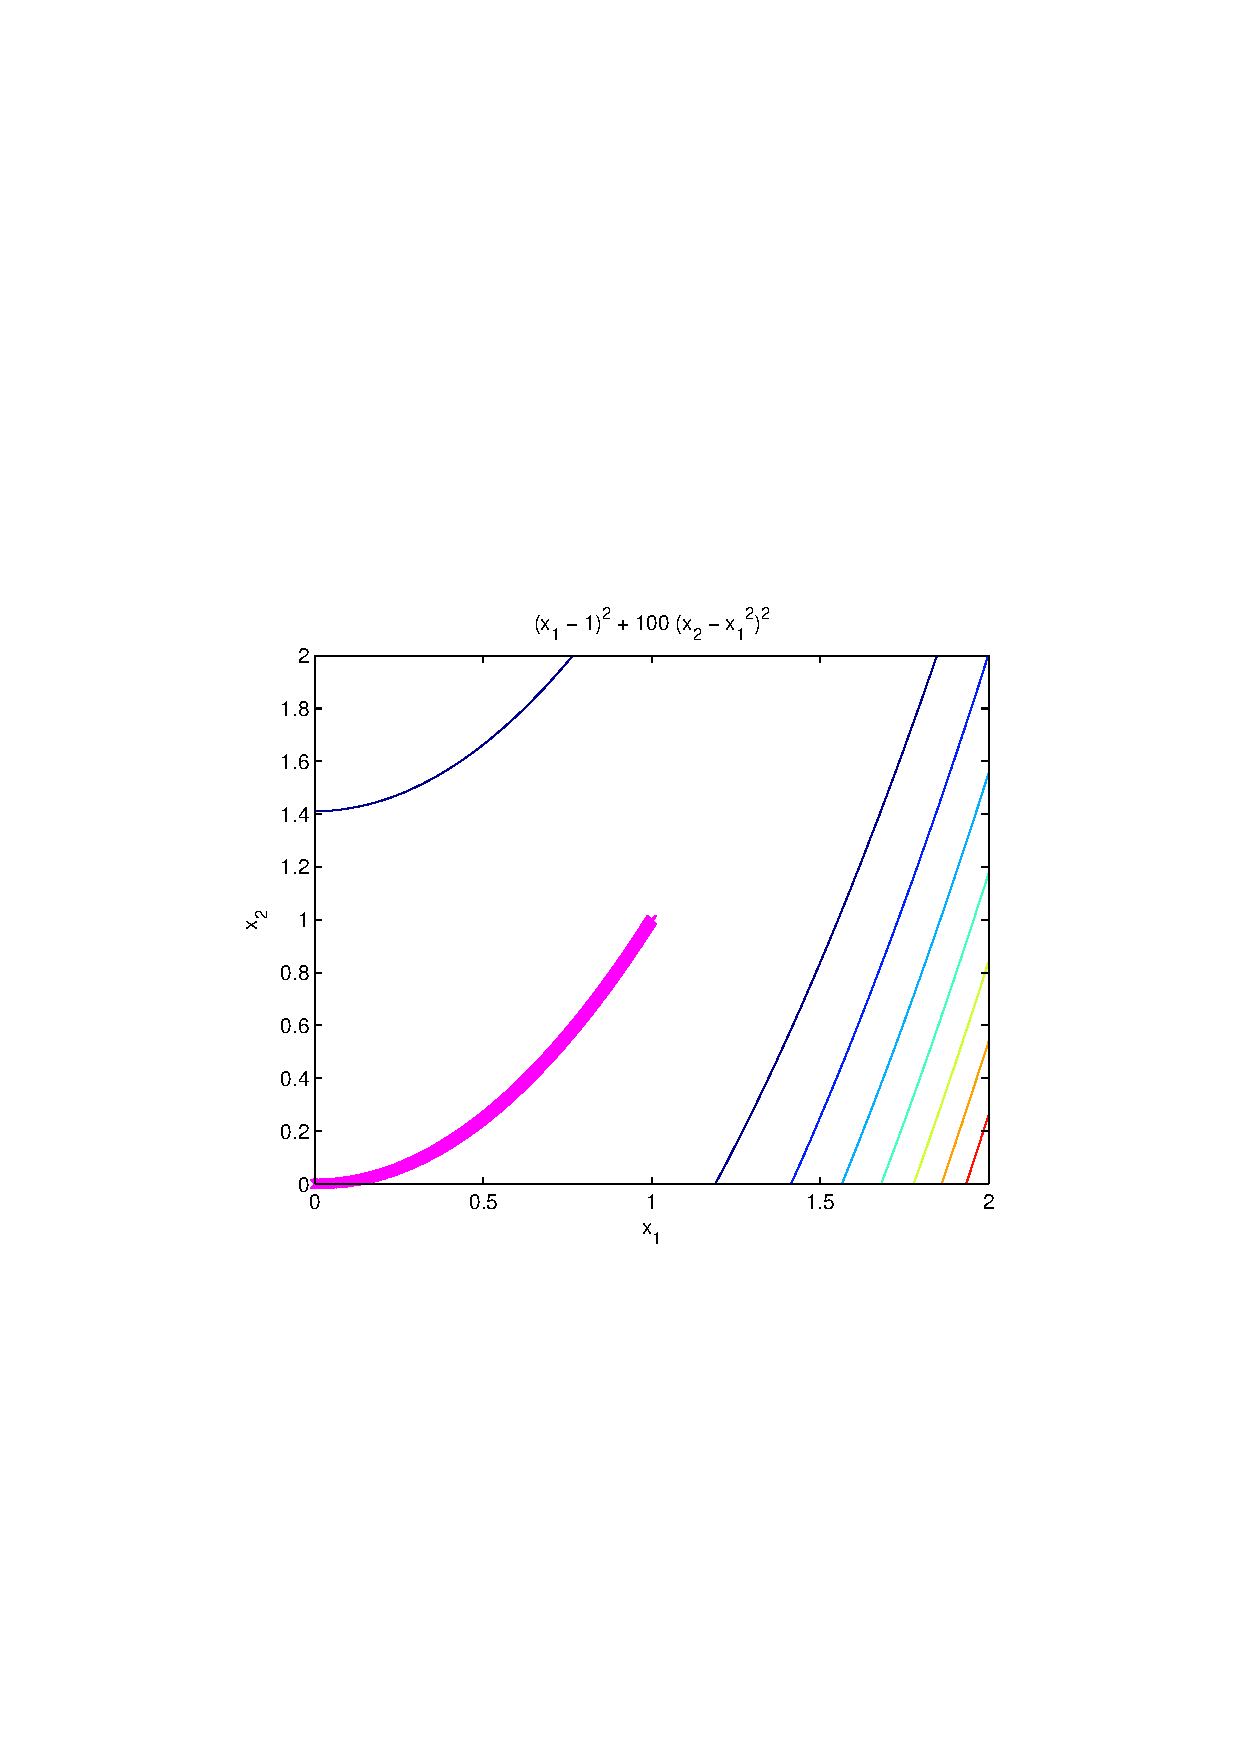
\includegraphics[width=\linewidth]{pic2.pdf}
      \caption{The switching curves $x_1(t)$ vs $x_2(t)$ passing through origin}
      \label{fig1} 
    \end{figure}
      \begin{figure}[h!]
      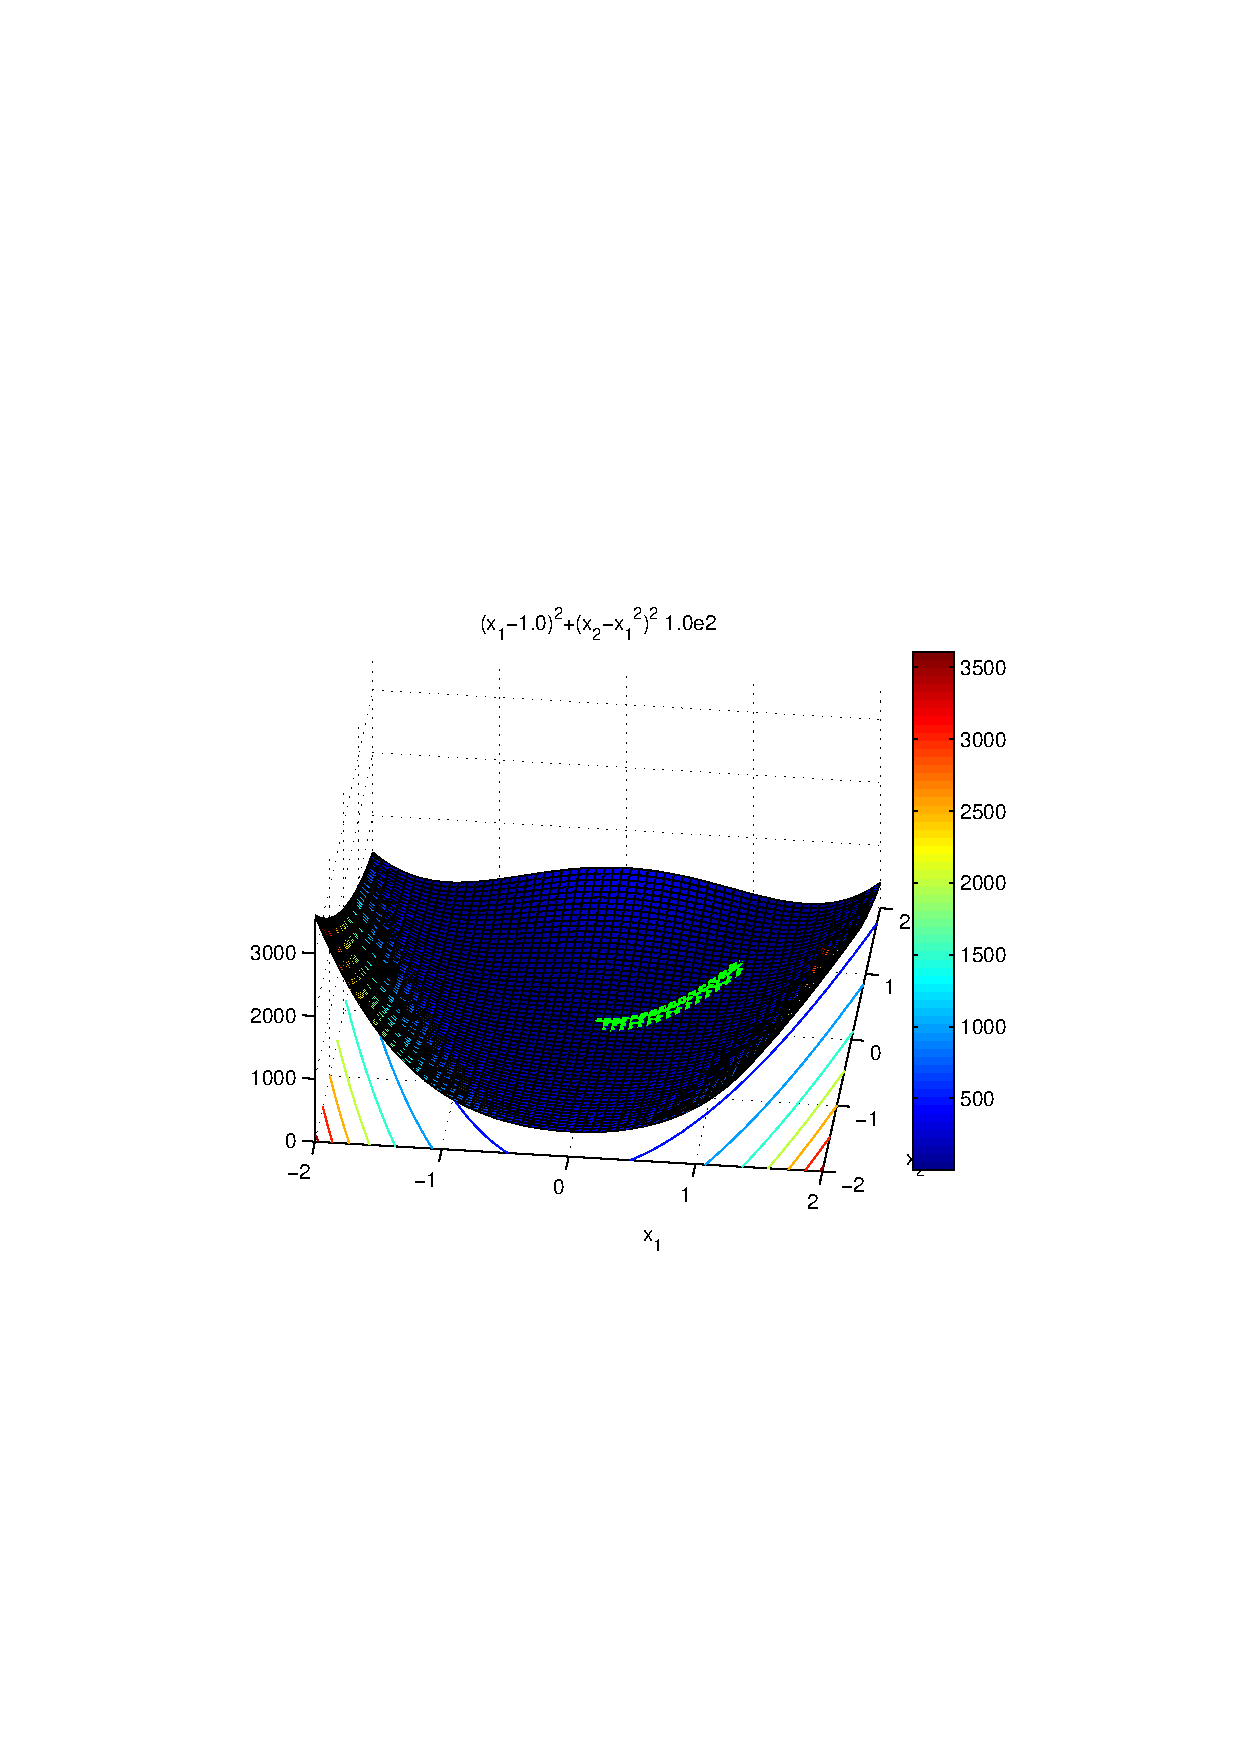
\includegraphics[width=\textwidth, height = 10cm, keepaspectratio= true]{pic1.pdf}
      \captionsetup{singlelinecheck=off}
      \caption{Plot of combined Family of curves (a) Red Lines show the family of u = -1 curves (b) Green Lines show the family of
u = 0 curves (b) Black Lines show the family of u = 1 curves (a = 2 for above curves)}
      \label{fig2} 
    \end{figure}
     \begin{figure}[h!]
      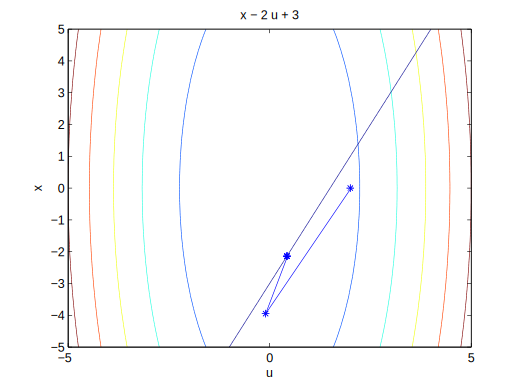
\includegraphics[width=\linewidth, height = 10cm,  keepaspectratio= tru]{pic3.pdf}
      \caption{Example Scenario 1 optimal control sequence(-1,0,1)}
      \label{fig3} 
    \end{figure}
    \begin{figure}[h!]
      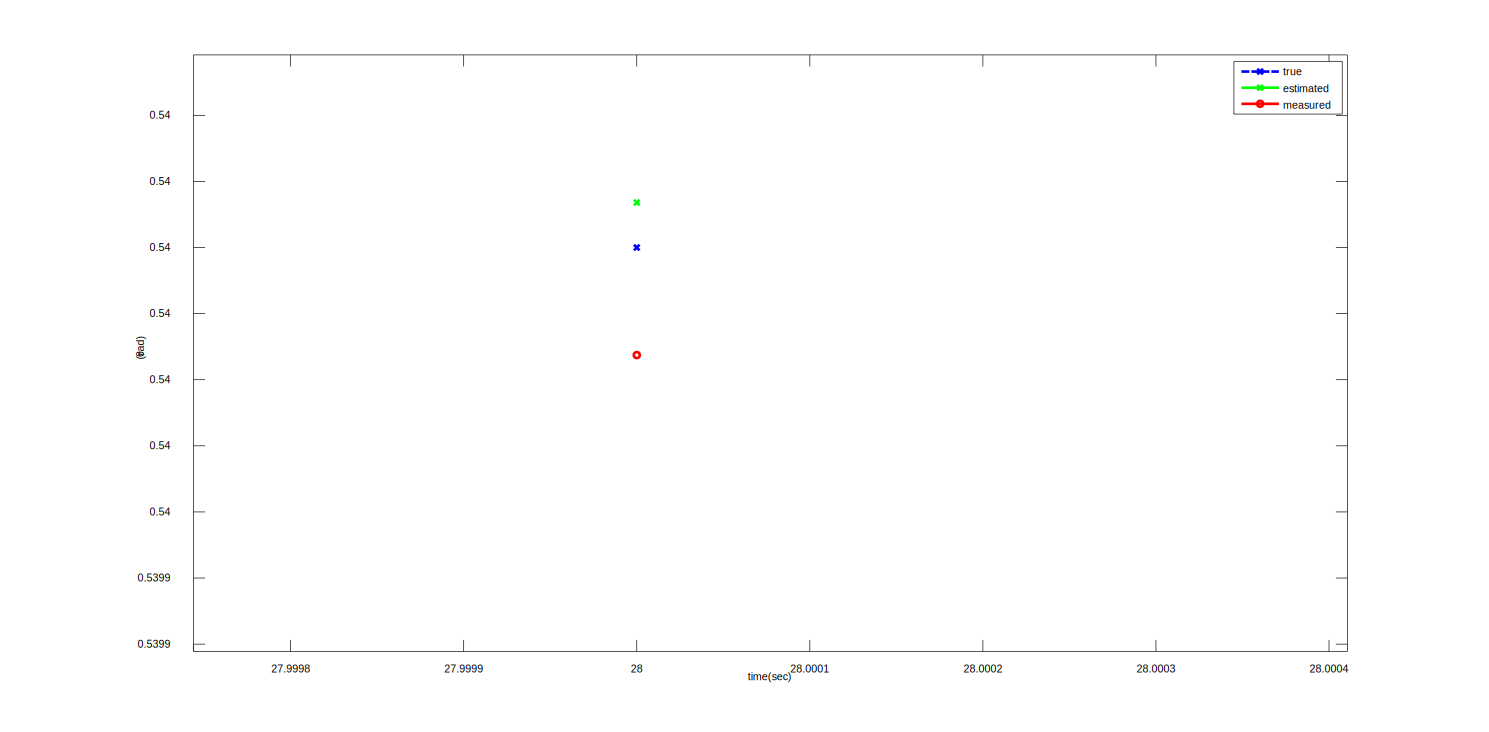
\includegraphics[width=\linewidth, height = 10cm,  keepaspectratio= tru]{pic4.pdf}
      \caption{Example Scenario 2 optimal control sequence(1,0,-1)}
      \label{fig4} 
    \end{figure}
    \newpage
  %%%%%%%%%%%%%%%Question 2%%%%%%%%%%%%%%%%%%%%%%%%
    \item Given to minimize:
      \begin{align*}
       J = \lVert x(t_f)\rVert^2 
      \end{align*}
      subjected to the dynamics of the system:
	\begin{align*}
	\dot x = Ax + Bu, \quad x(0) = x_0, \quad t_f \mbox{ given}
	\end{align*}
    Equating related parts of the problem to the general optimization setting, we have:
      \begin{align*}
       \Phi = x(t_f)^T x(t_f) \quad H = \lambda^T (Ax+Bu) 
      \end{align*}
      The necessary optimality conditions required are :
      \begin{align*}
       \dot \lambda &= - \nabla H_x = - A^T \lambda \\
       \partial H_u &= \lambda^T B\\
       \lambda(t_f) &= \nabla_x \Phi(t_f) = 2 x(t_f)
      \end{align*}
      Since the optimal control cannot be obtained by $\partial H_u$ we use poincare conditions to find the control on the
boundaries:
     \begin{align*}
      u^* &= argmin H^* (u) = \lambda^T B u\\
      \Rightarrow u^* &= \begin{cases}
                         -1 & \lambda^T B > 0\\
                         1 & \lambda^T B < 0\\
                         \mbox{singular} & \lambda^T B = 0
                        \end{cases}\\
     \end{align*}
     This shows that the control for optimization is bang bang i.e the control either stays at +1 or -1 if $\lambda^T B \neq0$.
     
     For the double integrator the dynamics of the system are given as follows:
       \begin{align*}
        A = \begin{bmatrix}
             0 & 1 \\
             0 & 0 \\
            \end{bmatrix} \quad 
        B = \begin{bmatrix}
             0 \\
             1
            \end{bmatrix}\\
       \end{align*}
       The control is then given as :
	 \begin{equation*}
	\Rightarrow u^* = \begin{cases}
                         -1 & \lambda_2 > 0\\
                         1 & \lambda_2 < 0\\
                         \mbox{singular} & \lambda_2 = 0
                        \end{cases}\\  
	 \end{equation*}
    Now to find the general trajectories for this case, we look at the system and multiplier dynamics. 
    \begin{align*}
    \dot \lambda_1 &= 0\\
    \dot \lambda_2  &= - \lambda_1\\
    \lambda(t_f) &= 2 x(t_f) \\
    \Rightarrow \lambda_1 &= \mbox{ const } \\
    \Rightarrow \lambda_2 &= -\lambda_1 t + c_1 \\
    \end{align*}
    The linearity of $\lambda_2$ implies that we can either switch once or not switch at all. But when $\lambda_2$ goes to zero we cannot decide on
the control since it is singular. Thus the possible optimal control sequences are $\{1\}, \{-1\}, \{1, -1\}, \{-1,1\}$.  

We explain the optimal control law based on one example scenario and then provide the general optimal control law after that. For 
example consider our starting condition to be $x_{0} < 0$(Third quadrant). Then the possible control sequences are $\{1\}$ or $\{1, -1\}$. The other sequences take you away from origin and are clearly not optimal.
In both the control sequences, we start with control u = 1. To choose the right sequence, we use the boundary conditions $\lambda(t_f) = x(t_f)$. If $t_f$ is less than the minimum time required to 
cross to fourth quadrant, then $x_2f < 0$. This implies that $\lambda_2f < 0$ and control $u_f = 1$. Thus the optimal sequence in this case is $u = 1$ throughout. In the case when $t_f$ is sufficient
to cross over to fourth quadrant, $x_2f > 0$ and $\lambda_2f > 0$. This implies $u_f = -1$ and the optimal control sequence is $\{1, -1\}$. In this way similar analysis can be done for other quadrants.

If the control is always +1 then initial position should lie on:
  \begin{align*}
   x_1(t_0) &= x_2(t_0)^2 \quad x_2(t_0) < 0 \\
   \mbox{OR } x_1(t_0) &< 0 , \enskip x_2(t_0) < 0 \quad \mbox{ (Third Quadrant with small } t_f)
  \end{align*}
else if the control is always -1 then initial position should lie on:
  \begin{align*}
   x_1(t0) &= -x_2(t_0)^2 \quad x_2(t_0) > 0\\
   \mbox{OR } x_1(t_0) &> 0 , \enskip x_2(t_0) > 0 \quad \mbox{ (First Quadrant with small } t_f)
  \end{align*}
else if the control sequence is \{-1,1\} then the initial position should lie in:
  \begin{align*}
   x_1(t_0) &> x_2(t_0)^2 \enskip x_2(t_0) < 0\\
   \mbox{OR } x_1(t_0) &> 0 , \enskip x_2(t_0) > 0 \quad \mbox{ (First Quadrant with large } t_f)
  \end{align*}
else if the control sequence is \{1,-1\} then the initial position should lie in:
  \begin{align*}
   x_1(t_0) &< -x_2(t_0)^2 \enskip x_2(t_0) > 0\\
   \mbox{OR } x_1(t_0) &< 0 , \enskip x_2(t_0) < 0 \quad \mbox{ (Third Quadrant with large } t_f)
  \end{align*}
(Here large $t_f$ is large enough to cross from one quadrant to another). It should be noted that, when $t_f $ is long enough to reach origin, we reach the least possible cost (0). So for every initial starting position, there is a $t_f^*$ above which the control law does not change.
%One important fact that makes this optimal control problem a lot simpler is that, when the time $t_f$ given is long enough to reach origin
%using any of the above sequences then we do not have to execute any more control since we already have reached the goal i.e least possible distance to origin. This fact
%implies that there is minimum final time for every position beyond which the control sequence does not change. 

The switching curves which go to zero are shown in Fig[\ref{fig5}] and the optimal trajectories for some of the sequences
discussed above are shown in Fig[\ref{fig6}]
  \begin{figure}[h!]
    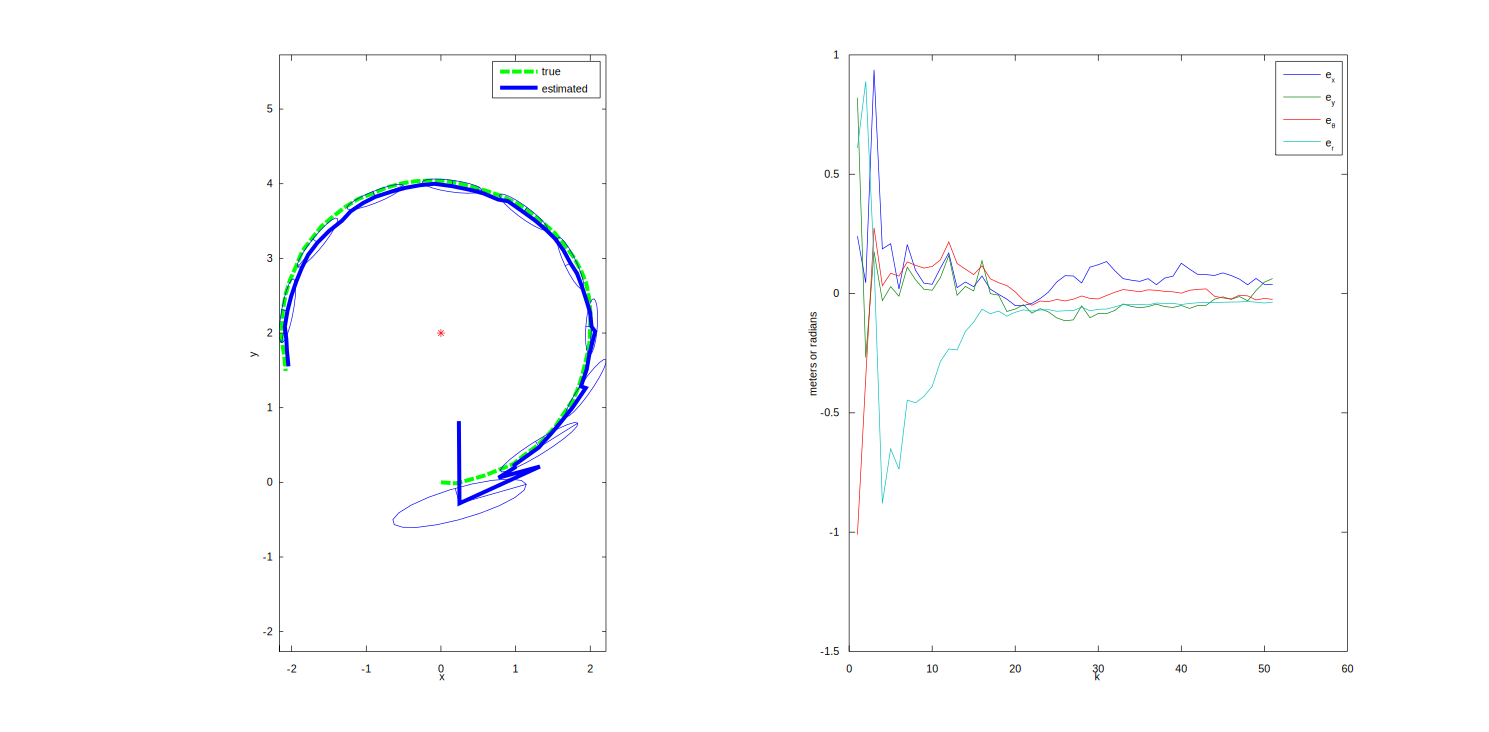
\includegraphics[width=\linewidth]{pic5.pdf}
    \caption{The switching curves $x_1(t)$ vs $x_2(t)$ passing through origin}
    \label{fig5} 
  \end{figure}
  \begin{figure}[h!]
    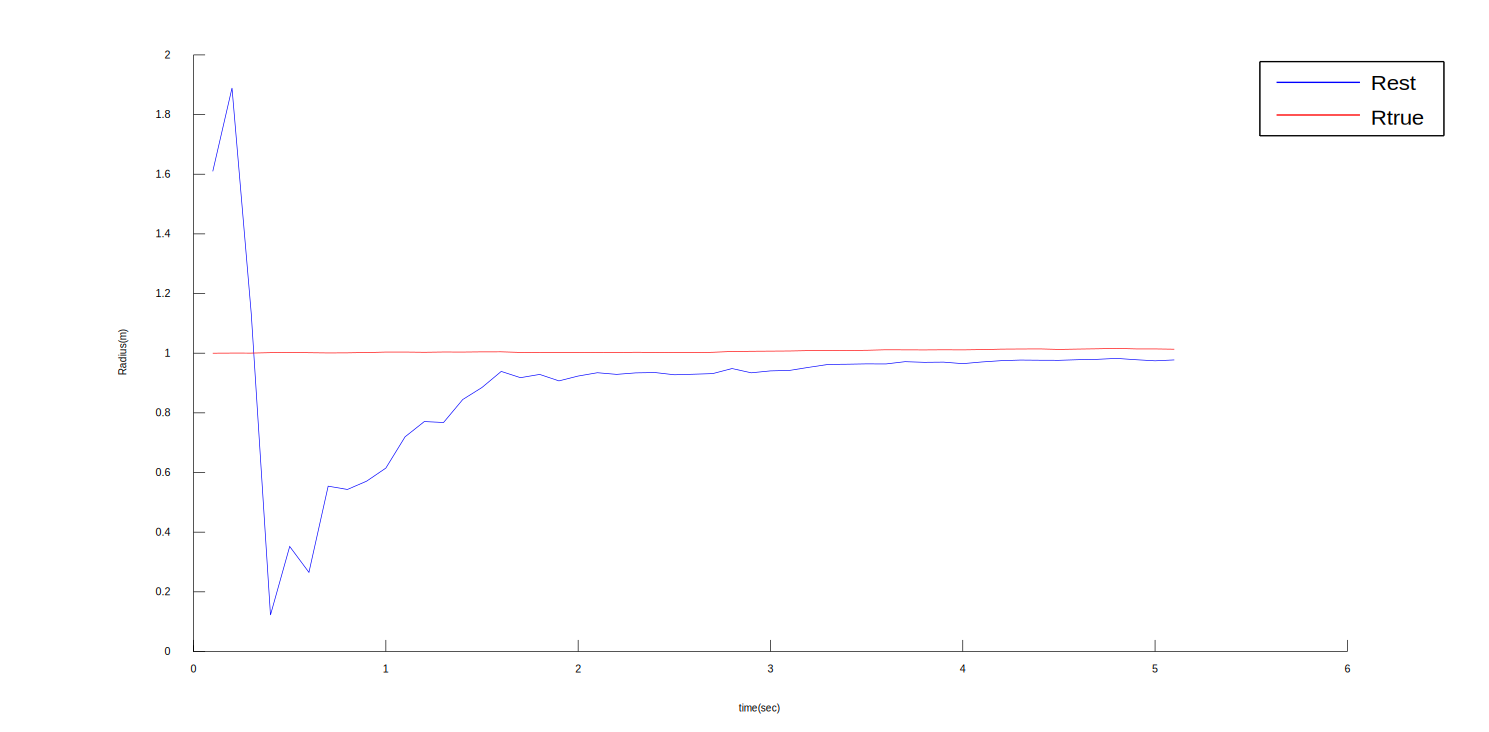
\includegraphics[width=\linewidth]{pic6.pdf}
    \caption{The optimal trajectories  $x_1(t)$ vs $x_2(t)$ depicting various control sequences plotted by simulating the
dynamics in MATLAB.(a) The red curves represent u = -1 and green represent u = +1 (b) Once the paths reach origin, they do not
move any further even if the final time is increased. The control remains zeros thereafter.}
    \label{fig6} 
  \end{figure}
%decide on the figures when u get time 

  %%%%%%%%%%%%%%%Question 3%%%%%%%%%%%%%%%%%%%%%%%%
\item Given a robotic arm with two degrees of freedom ($\theta_1, \theta_2$). The state of the arm is given as:
  \begin{equation*}
   x = (\theta_1, \theta_2, \dot \theta_1, \dot \theta_2)
  \end{equation*}
  The forward kinematics of the RR manipulator is given as:
    \begin{equation*}
     p_t = \begin{pmatrix}
            cos(\theta_1) l_1 + cos(\theta_1 + \theta_2) l_2 \\
            sin(\theta_1) l_1 + sin(\theta_1 + \theta_2) l_2 \\
           \end{pmatrix}
    \end{equation*}
   The state inequality for obstacle avoidance is given as:
     \begin{align*}
      \lVert p_t - p_0 \rVert^2 &\ge r^2 \\
      c(x(t),t) = r^2 - (p_t - p_0)^T (p_t - p_0) &\le 0 \\
     \end{align*}
    Since the above state inequality does not directly say anything about the control, we differentiate c(x(t),t) until controls
show up. Thus the new inequality are obtained as:
  

  \begin{align*}
  \dot c &= 2{(p_0-p_t)}^T \dot p_t  = 2{(p_0-p_t)}^T (\partial_x{p_t} \dot x) \\
  \mbox{Where } \partial_x p_t &= \begin{pmatrix}
                                  -sin(\theta_1)l_1 - sin(\theta_1 + \theta_2) l_2 & - sin(\theta_1 + \theta_2) l_2 & 0 & 0\\
                                  cos(\theta_1)l_1 + cos(\theta_1 + \theta_2) l_2 & cos(\theta_1 + \theta_2) l_2 & 0 & 0\\
                                 \end{pmatrix}\\
  \Rightarrow  \dot c &= 2(p_0 - p_t)^T \begin{pmatrix}
                                  -sin(\theta_1)l_1 \dot \theta_1 - sin(\theta_1 + \theta_2) l_2 (\dot \theta_1 + \dot \theta_2)\\
                                  cos(\theta_1)l_1 \dot \theta_1 + cos(\theta_1 + \theta_2) l_2 (\dot \theta_1 + \dot \theta_2)\\
                                       \end{pmatrix}\\
  \end{align*}
  Since $\dot c$  does not have information about u1 and u2 we differentiate again to get 
  \begin{align*}
   \ddot c &= 2(p_0 - p_t)^T(\partial_x(\partial_x p_t \dot x) \dot x) + 2 (\partial_x p_t \dot x)^T (\partial_x p_t \dot x)\\ 
  \partial_x(\partial_x p_t) &= \begin{pmatrix}
				    -l_1 cos(\theta_1) \dot \theta_1 - l_2 cos(\theta_1 + \theta_2)(\dot \theta_1 +
\dot \theta_2)& \cdots \\
 \hfill -l_2 cos(\theta_1 + \theta_2)  (\dot \theta_1 + \dot \theta_2) & -l_1 sin(\theta_1) -l_2sin(\theta_1 +
\theta_2) & -l_2sin(\theta_1+ \theta_2)\\[6pt]
                                  -l_1 sin(\theta_1) \dot \theta_1 - l_2 sin(\theta_1 + \theta_2)(\dot \theta_1 + \dot \theta_2)
& \cdots\\ 
\hfill -l_2 sin(\theta_1 + \theta_2)  (\dot \theta_1 + \dot \theta_2) &  l_1 cos(\theta_1) +  l_2cos(\theta_1 + \theta_2)
& l_2cos(\theta_1 + \theta_2)\\[6pt]
                                 \end{pmatrix}\\
   \partial_x(\partial_x p_t)\dot x &= \begin{pmatrix}
					-l_1 c_1 \dot \theta_1^2 -l_2 c_{12} (\dot \theta_1 + \dot \theta_2)^2 + u_1 (-l_1 s_1 -
l_2 s_{12}) + u_2 (-l_2 s_{12})\\
					-l_1 s_1 \dot \theta_1^2 -l_2 s_{12} (\dot \theta_1 + \dot \theta_2)^2 + u_1 (l_1 c_1 +
l_2 c_{12}) + u_2 (l_2 c_{12})\\
                                      \end{pmatrix}\\
   \partial_x p_t \dot x &= \begin{pmatrix}
                                  -sin(\theta_1)l_1 \dot \theta_1 - sin(\theta_1 + \theta_2) l_2 (\dot \theta_1 + \dot \theta_2)\\
                                  cos(\theta_1)l_1 \dot \theta_1 + cos(\theta_1 + \theta_2) l_2 (\dot \theta_1 + \dot \theta_2)\\
                                       \end{pmatrix}\\
  \end{align*}
 The above inequality has $u_1$ and $u_2$. Hence the collection $(c \enskip\dot c\enskip \ddot c) \le 0$ gives the state
control inequality conditions which must be satisfied on the boundary. Thus the constraints are:
  \begin{align*}
      c(x(t),t) &= r^2 - (p_t - p_0)^T (p_t - p_0) \le 0 \\
   \dot c(x(t),t) &= 2(p_0 - p_t)^T \begin{pmatrix}
                                  -sin(\theta_1)l_1 \dot \theta_1 - sin(\theta_1 + \theta_2) l_2 (\dot \theta_1 + \dot \theta_2)\\
                                  cos(\theta_1)l_1 \dot \theta_1 + cos(\theta_1 + \theta_2) l_2 (\dot \theta_1 + \dot \theta_2)\\
                                       \end{pmatrix} \le 0\\
    (p_0 - p_t)^T &\begin{bmatrix}
 -l_1 sin(\theta_1) -l_2sin(\theta_1 + \theta_2) & -l_2sin(\theta_1+ \theta_2)\\
  l_1 cos(\theta_1) +  l_2cos(\theta_1 + \theta_2) & l_2cos(\theta_1 + \theta_2)\\
                  \end{bmatrix} 
                  \begin{bmatrix}
                   u_1 \\
                   u_2 \\
                  \end{bmatrix} \le - (\partial_x p_t \dot x)^T (\partial_x p_t \dot x) - (p_0 - p_t)^T M(x)
  \end{align*}
\item Given rocket dynamics as :
\begin{align*}
 \dot x_1(t) &= \frac{cu(t)}{x_2(t)} - \frac{D}{x_2(t)} \\
 \dot x_2(t) &= - u(t) \\
\end{align*}
 To maximize the range of rocket, the optimization problem is set as:
 \begin{align*}
   \mbox{maximize }J = \int_{t_0}^{t_f} x_1(t) dt \quad x(t_0) \mbox{ and } x(t_f) \mbox{ are given}
 \end{align*}
 and terminal time is free. Equating to the general optimal control setting we get:
 \begin{align*}
  H = x_1(t) + \lambda_1( \frac{cu(t)}{x_2(t)} - \frac{D}{x_2(t)} ) + \lambda_2 ( - u(t)) \\
 \end{align*}
 Since terminal time is free and there are no terminal constraints, $H(t_f) = 0$ and since H is not explicitly dependent on time (t), H = const = 0 throught the interval.
 The adjoint equations for the control problem are given as:
 \begin{align*}
  \dot \lambda_1 &= - 1 \\
  \dot \lambda_2 &= -\lambda_1\left(\frac{cu - D}{{x_2}^2}\right)
 \end{align*}
 To investigate the possibility of singular control intervals, we try to find the necessary optimal conditions:
 \begin{align*}
  H_u = \frac{c \lambda_1}{x_2} - \lambda_2 = 0\\
 \end{align*}
 Since $H_u$ does not provide the optimal control directly, we check if we are on the boundaries.
 \begin{align*}
  \mbox{maximize }H^*(u) = \left(\frac{c \lambda_1}{x_2} - \lambda_2\right) u \\
 \end{align*}
 The boundary condition on u is given as $0 \le u(t) \le u_{m}$. Hence to maximize Hamiltonian, the Optimal control is given as:
 \begin{align*}
	      u =       \begin{cases}
                         u_m & \left(\frac{c \lambda_1}{x_2} - \lambda_2\right) > 0\\
                         0 & \left(\frac{c \lambda_1}{x_2} - \lambda_2\right)< 0\\
                         \mbox{singular} & \left(\frac{c \lambda_1}{x_2} - \lambda_2\right) = 0
                        \end{cases}\\ 
 \end{align*}
 
 To evaluate the possiblity of singular intervals, we want to evaluate the singular condition over a period of time. During the singular interval, 
 \begin{align*}
  \dot H_u &= \frac{-c \lambda_1}{{x_2}^2} (-u) + \frac{c(-1)}{x_2} - (-\lambda_1)\left(\frac{cu - D}{{x_2}^2}\right) = 0\\ 
  \Rightarrow \dot H_u &= \frac{-c}{x_2} + \frac{\lambda_1 D}{{x_2}^2} = 0\\
  \Rightarrow \lambda_1 &= \frac{c x_2}{D}\\ 
  \Rightarrow \ddot H_u &= \frac{c}{{x_2}^2} (-u) - \frac{2\lambda_1 D}{{x_2}^3}(-u) - \frac{D}{{x_2}^2} = 0\\
  \Rightarrow   u^* &= \frac{D x_2}{2 \lambda_1 D - c x_2  } = \frac{D}{c}
 \end{align*}
 So if the fuel burn rate is constant at $\frac{D}{c}$, and $\lambda_1 = c \frac{x_2}{D}$, and $\lambda_2 = \frac{c^2}{D}$ for some period of time, then that interval is a singular interval. But if $\frac{D}{c}$ is greater than 
 $u_m$, then we do not have a singular interval.

\end{enumerate} 
\vfill
\begin{acknowledgements}
I hereby declare that I have not discussed this homework with anyone. The solutions written here are
my own work and  from lecture notes and sample code provided by the professor. Any 
external references are mentioned in the text.
\flushright Gowtham Garimella
\end{acknowledgements}




\end{document}
